\chapter{Odoo Sous Docker}

	Dans ce qui suit, nous allons donner une idée sur l'interface que fournit Docker pour la provision des services (conteneurs). Nous allons réalisé la mini-architecture suivante:
	
	\begin{figure}[H]
	\centering
	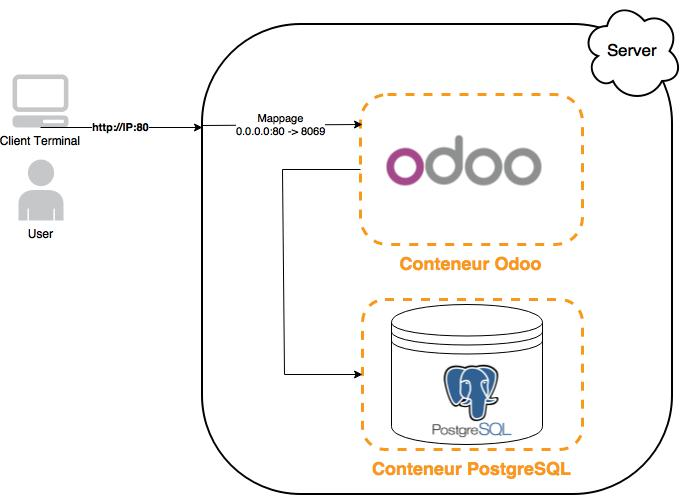
\includegraphics [scale=0.5]{biblio/odoo.jpg}
	\caption{Odoo sous Docker}
	\label{fig:}
	\end{figure}

\section*{Environnement technique}
	
	On va partir d'un serveur Ubuntu 14.04-64 bits avec Docker installé (L'installation ne sera pas détaillé), ou de préférence, un serveur CoreOS où Docker est déja inclut avec ce système d'éxploitation. A noter que Docker nécéssite un linux 64 bits avec un noyau >= 3.8.


\section*{Installation de PostgreSQL}

	Odoo a besoin d'un serveur de base de donnée PostgreSQL, la commande suivante permet de l'installer:

	\begin{lstlisting}[caption=Installation de PostgreSQL]
		$ docker run -d -e POSTGRES_USER=odoo -e POSTGRES_PASSWORD=odoo --name db postgres
	\end{lstlisting}




\section*{Installation d'Odoo}

	L'installation d'Odoo se fait grâce à la commande suivante:
	\begin{lstlisting}[language=bash,caption=Installation d'Odoo]
		$ docker run -p 80:8069 --name odoo --link db:db -t odoo
	\end{lstlisting}

	En quelques secondes, on pu lancer le service Odoo prêt à être utilisé, personnalisé, et éventuellement porté vers un autre serveur. Pour accéder au service il suffit de taper dans le navigateur:

	\begin{lstlisting}[language=bash]
		http://IP_SERVEUR:80
	\end{lstlisting}

	




\chapter{Docker-compose}

	On va réaliser l'installation détaillé dans \emph{l'Annexe A} avec l'outil \emph{Docker-compose}. Cet outil permet de définir dans un fichier \acrshort{yaml} l'architecture de l'application. Enfin, on peut faire des manipulation (démarrage, redémarrage, arrêt) sur toute l'architecture comme si c'était un seul service.

	\begin{lstlisting}[language=bash,caption=Installation d'Odoo avec Docker-compose]
		odoo:
	  		image: odoo
		  	links:
		   		- db
		  	ports:
		   		- "80:8069"
		db:
		  	image: postgres
		  	environment:
  				- POSTGRES_USER: odoo
  				- POSTGRES_PASSWORD: odoo
	\end{lstlisting}

	\begin{lstlisting}[language=bash,caption=Lancement d'Odoo avec Docker-compose]
		$ docker-compose up -d
	\end{lstlisting}



\chapter{Douze-facteurs d'un SaaS}
\label{annexe:12factors}
\index{Douze-facteurs}

Dans l'informatique moderne, le logiciel est généralement livré comme un service: appelés \acrshort{saas}. Les douze-facteurs d'un SaaS est une méthodologie pour la création d'application qui:

\begin{itemize}
	\item Réduit le temps et le coût pour les nouveaux développeurs participant au projet;
	\item offre une \textbf{portabilité maximale} entre les environnements d'exécution;
	\item Sont appropriées pour le \textbf{déploiement} sur les \textbf{plates-formes de cloud} modernes, éliminant ainsi la nécessité de serveurs et d'administration de systèmes;
	\item \textbf{Réduit la divergence} entre le développement et la production, permettant un déploiement continu;
	\item peut \textbf{monter en charge} sans toucher aux outils, à l'architecture, ou à les pratiques de développement.
\end{itemize}


La méthodologie des douze-facteurs synthétise l'éxpérience de l'équipe de Heroku, un des tout premiers services cloud \cite{12-factors}. Elles peut être appliquée à des applications écrites dans n'importe quel langage de programmation, et qui sont combinées à n'importe quel services (base de données, file d'attente, mémoire cache, etc.).


\section*{code source}

Le code source de l'application doit être unique mis et suivi depuis un système de contrôle de version comme Git.

\section*{Dépendances}

La plupart des langages de programmation un sytème de gestion de dépendances. Ainsi, une application doit déclarer explicitement et isoler les dépendances. Un SaaS robuste ne repose jamais sur l'éxistence implicite des dépendances. 

\section*{Configuration}

Les variables de configurations peuvent varier entre les environnements (développement, test, production, etc). Ces variables ne doivent jamais être stockées dans des constantes à l'intérieur du code. Une bonne pratique c'est les stocker dans des variables d'environnement.

\section*{Services de support}

Traiter tous les services de support (base de données, file d'attente, serveur \acrshort{smtp}, etc.)  comme des ressources liées.

\section*{Build, release, run}

Pour déployer une application, il faut passer par trois étapes:
\begin{itemize}
	\item build: transformer le code source en exécutable;
	\item release: combiner l'exécutable avec les configurations;
	\item run: lancer les processus dans l'environnement d'exécution .
\end{itemize}


\section*{Processus}

Les processus d'une application doivent être \textbf{sans état} (stateless). Les données persistentes doivent être stockées dans une base de donnée.

\section*{Attachement de port}

Chaque service doit être exporté via un port.

\section*{Concurrence}

Les processus d'une application ne doivent jamais lancés comme un démon. Au lieu de cela,il faut compter sur le gestionnaire de processus du système d'exploitation (systemd, init.d, upstart, etc.).

\section*{Jetable}

Les processus d'une application sont jetables, ils peuvent être stoppés ou démarrés à n'importe quel moment rapidement et sans causer de problèmes.

\section*{Parité Dev/Prod}

Il faut garder tous les environnements (développement, test, production, etc) similaires.

\section*{Messages logs}

Les messages logs sont très importants, il faut les traiter comme des flux d'événements.

\section*{Processus admin}

Les tâches d'administration doivent être exécutés dans un unique processus avec un environnement identique à celui du processus principal. 

\chapter{Fournisseurs du Cloud}

\section*{Amazon Web Services}
\index{AWS}

\acrshort{aws} est une collection de services informatiques distants fournis via internet par le groupe américain de commerce électronique Amazon.com. Lancé officiellement en 2006, Amazon Web Services fournit des services en lignes à d'autres sites internet ou applications clientes. La plupart d'entre eux ne sont pas directement exposés à l'utilisateur final, mais offrent des fonctionnalités que d'autres développeurs peuvent utiliser. Parmi les services qu'offre \acrshort{aws}, on trouve Elastic Compute Cloud (EC2), fournissant des serveurs virtuels évolutifs utilisant Xen. 

\acrshort{aws} offre aux nouveaux clients une version d'évaluation de 12 mois, ce qui a permit d'utiliser le service EC2 dans ce projet pour créer un cluster de trois serveurs.

\section*{Google Compute Engine}
\index{GCE}

Google est présent depuis de nombreuses années sur les services \acrshort{saas} et \acrshort{paas} via Google Apps et Google App Engine. Ce n'est qu'en décembre 2013 que Google a fait son entrée sur le marché du \acrshort{iaas} avec une version finale.

Sur le marché du IaaS, Amazon EC2 est aujourd'hui la référence en termes de nombre d'utilisateurs, de qualité de service et de fonctionnalités, mais Google a fait une entrée assez fracassante avec une offre qui dépasse déjà le reste du marché. En effet, Google propose une volumétrie de stockage plus importante, une meilleure bande passante ainsi qu'un temps de démarrage des machines virtuelles optimisé.

\acrshort{gce} offre aux nouveaux clients 300 dollars virtuels à consommer au moins de 2 mois. Ce qui a permit d'essayer cette \acrshort{iaas} dans ce projet pour créer un cluster où Deis a été installé.

\section*{Heroku}
\index{Heroku}

Heroku est un service de cloud computing de type plate-forme en tant que service. Créé en 2007, il était l'un des tout premiers services cloud, puis a été racheté par Salesforce.com. Cette plate-forme est destinée pour les développeurs pour y mettre leurs applications programmées dans la plupart des technologies web.

Hereku n'est pas utilisé durant notre projet, mais il a influencé le projet indirectement. En effet, Heroku a tellement inspiré Deis de sorte qu'elle a été décrite comme un mini-Heroku privé. Par ailleurs, l'équipe de Heroku a résumé son expérience dans la scalabilité des applications et a introduit les douze-éléments d'un \acrshort{saas}

%\chapter{Ordonnancement avec Fleet}